        %%******************************************%%
        %%                                          %%
        %%        Modello di tesi di laurea         %%
        %%            di Andrea Giraldin            %%
        %%                                          %%
        %%             2 novembre 2012              %%
        %%                                          %%
        %%******************************************%%


% I seguenti commenti speciali impostano:
% 1. 
% 2. PDFLaTeX come motore di composizione;
% 3. tesi.tex come documento principale;
% 4. il controllo ortografico italiano per l'editor.

% !TEX encoding = UTF-8
% !TEX TS-program = pdflatex
% !TEX root = tesi.tex
% !TEX spellcheck = it-IT

\documentclass[10pt,                    % corpo del font principale
               a4paper,                 % carta A4
               twoside,                 % impagina per fronte-retro
               openright,               % inizio capitoli a destra
               english,                 
               italian,                 
               ]{book}    

%**************************************************************
% Importazione package
%************************************************************** 

%\usepackage{amsmath,amssymb,amsthm}    % matematica

\usepackage[T1]{fontenc}                % codifica dei font:
                                        % NOTA BENE! richiede una distribuzione *completa* di LaTeX

\usepackage[utf8]{inputenc}             % codifica di input; anche [latin1] va bene
                                        % NOTA BENE! va accordata con le preferenze dell'editor

\usepackage[english, italian]{babel}    % per scrivere in italiano e in inglese;
                                        % l'ultima lingua (l'italiano) risulta predefinita

\usepackage{bookmark}                   % segnalibri

\usepackage{caption}                    % didascalie

\usepackage{chngpage,calc}              % centra il frontespizio

\usepackage{csquotes}                   % gestisce automaticamente i caratteri (")

\usepackage{emptypage}                  % pagine vuote senza testatina e piede di pagina

\usepackage{epigraph}			% per epigrafi

\usepackage{eurosym}                    % simbolo dell'euro

%\usepackage{indentfirst}               % rientra il primo paragrafo di ogni sezione

\usepackage{graphicx}                   % immagini

\usepackage{hyperref}                   % collegamenti ipertestuali

\usepackage[binding=5mm]{layaureo}      % margini ottimizzati per l'A4; rilegatura di 5 mm

\usepackage{listings}                   % codici

\usepackage{microtype}                  % microtipografia

\usepackage{mparhack,fixltx2e,relsize}  % finezze tipografiche

\usepackage{nameref}                    % visualizza nome dei riferimenti                                      

\usepackage[font=small]{quoting}        % citazioni

\usepackage{subfig}                     % sottofigure, sottotabelle

\usepackage[italian]{varioref}          % riferimenti completi della pagina

\usepackage[dvipsnames]{xcolor}         % colori

\usepackage{booktabs}                   % tabelle                                       
\usepackage{tabularx}                   % tabelle di larghezza prefissata                                    
\usepackage{longtable}                  % tabelle su più pagine                                        
\usepackage{ltxtable}                   % tabelle su più pagine e adattabili in larghezza


\usepackage[toc, acronym]{glossaries}   % glossario
                                        % per includerlo nel documento bisogna:
                                        % 1. compilare una prima volta tesi.tex;
                                        % 2. eseguire: makeindex -s tesi.ist -t tesi.glg -o tesi.gls tesi.glo
                                        % 3. eseguire: makeindex -s tesi.ist -t tesi.alg -o tesi.acr tesi.acn
                                        % 4. compilare due volte tesi.tex.


\usepackage{cite,hyperref}
                                        % eccellente pacchetto per la bibliografia; 
                                        % produce uno stile di citazione autore-anno; 
                                        % lo stile "numeric-comp" produce riferimenti numerici
                                        % per includerlo nel documento bisogna:
                                        % 1. compilare una prima volta tesi.tex;
                                        % 2. eseguire: biber tesi
                                        % 3. compilare ancora tesi.tex.
                                 
                                 
\usepackage{placeins}
                                        
%**************************************************************
% file contenente le impostazioni della tesi
%**************************************************************

%**************************************************************
% Frontespizio
%**************************************************************

% Autore
\newcommand{\myName}{Ludovico Brocca}                                    
\newcommand{\myTitle}{Studio del Back-end a microservizi e implementazione del Front-End in Angular nel progetto web SyncRec}

% Tipo di tesi                   
\newcommand{\myDegree}{Tesi di laurea triennale}

% Università             
\newcommand{\myUni}{Università degli Studi di Padova}

% Facoltà       
\newcommand{\myFaculty}{Corso di Laurea in Informatica}

% Dipartimento
\newcommand{\myDepartment}{Dipartimento di Matematica "Tullio Levi-Civita"}

% Titolo del relatore
\newcommand{\profTitle}{Prof.}

% Relatore
\newcommand{\myProf}{Claudio Palazzi}

% Luogo
\newcommand{\myLocation}{Padova}

% Anno accademico
\newcommand{\myAA}{2018-2019}

% Data discussione
\newcommand{\myTime}{Settembre 2019}

\newcommand{\bookingEngine}{\textit{Booking Engine}}

%**************************************************************
% Impostazioni di impaginazione
% see: http://wwwcdf.pd.infn.it/AppuntiLinux/a2547.htm
%**************************************************************

\setlength{\parindent}{14pt}   % larghezza rientro della prima riga
\setlength{\parskip}{0pt}   % distanza tra i paragrafi




%**************************************************************
% Impostazioni di caption
%**************************************************************
\captionsetup{
    tableposition=top,
    figureposition=bottom,
    font=small,
    format=hang,
    labelfont=bf
}

%**************************************************************
% Impostazioni di glossaries
%**************************************************************

%**************************************************************
% Acronimi
%**************************************************************
\renewcommand{\acronymname}{Acronimi e abbreviazioni}


\newacronym[description={\glslink{umlg}{Unified Modeling Language}}]
    {uml}{UML}{Unified Modeling Language}

%**************************************************************
% Glossario
%**************************************************************
%\renewcommand{\glossaryname}{Glossario}

\newglossaryentry{incremento}
{
    name=\glslink{incremento}{Incremento},
    text=incremento,
    sort=incremento,
    description={Procedere per aggiunta ad una base},
    plural=incrementi
}

\newglossaryentry{Spring} 
{
	name=\glslink{spring}{Spring},
	text=Spring,
	sort=Spring,
	description={Framework  Java fortemente basato sul principio di Inversion of Control, fornisce uno stack di librerie molto versatile per lo sviluppo di applicazioni Java},
	plural=incrementi
}

\newglossaryentry{ERP}
{
	name=\glslink{erp}{ERP},
	text=ERP,
	sort=ERP,
	description={TODO},
	plural=ERP,
}

\newglossaryentry{ICT} {
	name=\glslink{ict}{ICT},
	text=ICT,
	sort=ICT,
	description={TODO},
	plural=ICT,
}

\newglossaryentry{System Integrator}
{
	name=\glslink{system integrator}{System Integrator},
	text=System Integrator,
	sort=System Integrator,
	description={TODO},
	plural=System Integrators,
}

\newglossaryentry{iterazione}
{
    name=\glslink{iterazione}{Iterazione},
    text=iterazione,
    sort=iterazione,
    description={Procedere per rivisitazioni (può includere un incremento o addirittura un decremento).\\L'iterazione è un processo di durata non determinabile (anche potenzialmente infinita)},
    plural=iterazioni
}

\newglossaryentry{api}{
	name={\glslink{api}{api}},
	description={description}
}
 % database di termini
\makeglossaries


%**************************************************************
% Impostazioni di graphicx
%**************************************************************
\graphicspath{{immagini/}} % cartella dove sono riposte le immagini


%**************************************************************
% Impostazioni di hyperref
%**************************************************************
\hypersetup{
    %hyperfootnotes=false,
    %pdfpagelabels,
    %draft,	% = elimina tutti i link (utile per stampe in bianco e nero)
    colorlinks=true,
    linktocpage=true,
    pdfstartpage=1,
    pdfstartview=FitV,
    % decommenta la riga seguente per avere link in nero (per esempio per la stampa in bianco e nero)
    %colorlinks=false, linktocpage=false, pdfborder={0 0 0}, pdfstartpage=1, pdfstartview=FitV,
    breaklinks=true,
    pdfpagemode=UseNone,
    pageanchor=true,
    pdfpagemode=UseOutlines,
    plainpages=false,
    bookmarksnumbered,
    bookmarksopen=true,
    bookmarksopenlevel=1,
    hypertexnames=true,
    pdfhighlight=/O,
    %nesting=true,
    %frenchlinks,
    urlcolor=webbrown,
    linkcolor=RoyalBlue,
    citecolor=webgreen,
    %pagecolor=RoyalBlue,
    %urlcolor=Black, linkcolor=Black, citecolor=Black, %pagecolor=Black,
    pdftitle={\myTitle},
    pdfauthor={\textcopyright\ \myName, \myUni, \myFaculty},
    pdfsubject={},
    pdfkeywords={},
    pdfcreator={pdfLaTeX},
    pdfproducer={LaTeX}
}

%**************************************************************
% Impostazioni di itemize
%**************************************************************
%\renewcommand{\labelitemi}{$\ast$}lhead

\renewcommand{\labelitemi}{$\bullet$}
%\renewcommand{\labelitemii}{$\cdot$}
%\renewcommand{\labelitemiii}{$\diamond$}
%\renewcommand{\labelitemiv}{$\ast$}


%**************************************************************
% Impostazioni di listings
%**************************************************************
\lstset{
    language=[LaTeX]Tex,%C++,
    keywordstyle=\color{RoyalBlue}, %\bfseries,
    basicstyle=\small\ttfamily,
    %identifierstyle=\color{NavyBlue},
    commentstyle=\color{Green}\ttfamily,
    stringstyle=\rmfamily,
    numbers=none, %left,%
    numberstyle=\scriptsize, %\tiny
    stepnumber=5,
    numbersep=8pt,
    showstringspaces=false,
    breaklines=true,
    frameround=ftff,
    frame=single
} 


%**************************************************************
% Impostazioni di xcolor
%**************************************************************
\definecolor{webgreen}{rgb}{0,.5,0}
\definecolor{webbrown}{rgb}{.6,0,0}


%**************************************************************
% Altro
%**************************************************************

\newcommand{\omissis}{[\dots\negthinspace]} % produce [...]

% eccezioni all'algoritmo di sillabazione
\hyphenation
{
    ma-cro-istru-zio-ne
    gi-ral-din
}

\newcommand{\sectionname}{sezione}
\addto\captionsitalian{\renewcommand{\figurename}{Figura}
                       \renewcommand{\tablename}{Tabella}}

\newcommand{\glsfirstoccur}{\ap{{[g]}}}

\newcommand{\intro}[1]{\emph{\textsf{#1}}}

%**************************************************************
% Environment per ``rischi''
%**************************************************************
\newcounter{riskcounter}                % define a counter
\setcounter{riskcounter}{0}             % set the counter to some initial value

%%%% Parameters
% #1: Title
\newenvironment{risk}[1]{
    \refstepcounter{riskcounter}        % increment counter
    \par \noindent                      % start new paragraph
    \textbf{\arabic{riskcounter}. #1}   % display the title before the 
                                        % content of the environment is displayed 
}{
    \par\medskip
}

\newcommand{\riskname}{Rischio}

\newcommand{\riskdescription}[1]{\textbf{\\Descrizione:} #1.}

\newcommand{\risksolution}[1]{\textbf{\\Soluzione:} #1.}

%**************************************************************
% Environment per ``use case''
%**************************************************************
\newcounter{usecasecounter}             % define a counter
\setcounter{usecasecounter}{0}          % set the counter to some initial value

%%%% Parameters
% #1: ID
% #2: Nome
\newenvironment{usecase}[2]{
    \renewcommand{\theusecasecounter}{\usecasename #1}  % this is where the display of 
                                                        % the counter is overwritten/modified
    \refstepcounter{usecasecounter}             % increment counter
    \vspace{10pt}
    \par \noindent                              % start new paragraph
    {\large \textbf{\usecasename #1: #2}}       % display the title before the 
                                                % content of the environment is displayed 
    \medskip
}{
    \medskip
}

\newcommand{\usecasename}{UC}

\newcommand{\usecaseactors}[1]{\textbf{\\Attori Principali:} #1. \vspace{4pt}}
\newcommand{\usecasepre}[1]{\textbf{\\Precondizioni:} #1. \vspace{4pt}}
\newcommand{\usecasedesc}[1]{\textbf{\\Descrizione:} #1. \vspace{4pt}}
\newcommand{\usecasepost}[1]{\textbf{\\Postcondizioni:} #1. \vspace{4pt}}
\newcommand{\usecasealt}[1]{\textbf{\\Scenario Alternativo:} #1. \vspace{4pt}}

%**************************************************************
% Environment per ``namespace description''
%**************************************************************

\newenvironment{namespacedesc}{
    \vspace{10pt}
    \par \noindent                              % start new paragraph
    \begin{description} 
}{
    \end{description}
    \medskip
}

\newcommand{\classdesc}[2]{\item[\textbf{#1:}] #2}

%\bibliography{bibliografia}                     % file con le impostazioni personali

\begin{document}
%**************************************************************
% Materiale iniziale
%**************************************************************
\frontmatter
% !TEX encoding = UTF-8
% !TEX TS-program = pdflatex
% !TEX root = ../tesi.tex

%**************************************************************
% Frontespizio 
%**************************************************************
\begin{titlepage}

\begin{center}

\begin{LARGE}
\textbf{\myUni}\\
\end{LARGE}

\vspace{10pt}

\begin{Large}
\textsc{\myDepartment}\\
\end{Large}

\vspace{10pt}

\begin{large}
\textsc{\myFaculty}\\
\end{large}

\vspace{25pt}
\begin{figure}[htbp]
\begin{center}

\includegraphics[height=6cm]{logo-unipd}
\end{center}
\end{figure}
\vspace{26pt} 

\begin{LARGE}
\begin{center}
\textbf{\myTitle}\\
\end{center}
\end{LARGE}

\vspace{10pt} 

\begin{large}
\textsl{\myDegree}\\
\end{large}

\vspace{30pt} 

\begin{large}
\begin{flushleft}
\textit{Relatore}\\ 
\vspace{5pt} 
\profTitle\hphantom{i}\myProf
\end{flushleft}

\vspace{0pt} 

\begin{flushright}
\textit{Laureando}\\ 
\vspace{5pt} 
\myName
\end{flushright}
\end{large}

\vspace{40pt}

\line(1, 0){338} \\
\begin{normalsize}
\textsc{Anno Accademico \myAA}
\end{normalsize}

\end{center}
\end{titlepage} 
% !TEX encoding = UTF-8
% !TEX TS-program = pdflatex
% !TEX root = ../tesi.tex

%**************************************************************
% Colophon
%**************************************************************
\clearpage
\phantomsection
\thispagestyle{empty}

\hfill

\vfill

\noindent\myName: \textit{\myTitle,}
\myDegree,
\textcopyright\ \myTime.
%% !TEX encoding = UTF-8
% !TEX TS-program = pdflatex
% !TEX root = ../tesi.tex

%**************************************************************
% Dedica
%**************************************************************
\cleardoublepage
\phantomsection
\thispagestyle{empty}
\pdfbookmark{Dedica}{Dedica}

\vspace*{3cm}

\begin{center}
Lorem ipsum dolor sit amet, consectetuer adipiscing elit. \\ \medskip
--- Oscar Wilde    
\end{center}

\medskip

\begin{center}
Dedicato a ...
\end{center}

%% !TEX encoding = UTF-8
% !TEX TS-program = pdflatex
% !TEX root = ../tesi.tex

%**************************************************************
% Sommario
%**************************************************************
\cleardoublepage
\phantomsection
\pdfbookmark{Sommario}{Sommario}
\begingroup
\let\clearpage\relax
\let\cleardoublepage\relax
\let\cleardoublepage\relax

\chapter*{Sommario}

Il presente documento relaziona il risultato del lavoro prodotto a seguito del periodo di stage formativo svolto dal laureando Ludovico Brocca presso l'azienda SyncLab s.r.l., della durata di circa trecento ore.\\
Prima dell'inizio dell'attività di lavoro, sono stati concordati degli obiettivi con il tutor aziendale dr. Fabio Pallaro e con il relatore prof. Claudio Palazzi.\\
Tali obbiettivi prevedevano un periodo iniziale di formazione su tecnologie in uso presso l'azienda e di particolare interesse personale, a cui poi è seguita l'implementazione di un Front-End per una nuova versione di un applicativo, utilizzato per registrare le persone richiedenti un periodo di formazione presso l'azienda.\\
Lo scopo è stato fornire un prodotto in grado di sostituire la versione precedente, ormai datata, implementando un back-end a microservizi e un front-end in Angular 8.\\
Il lavoro è stato svolto in collaborazione con altri studenti aventi il periodo di stage formativo presso l'azienda; ciò ha permesso l'adozione di metodologie AGILE/ Scrum e il raggiungimento di una maggiore comprensione della prospettiva lavorativa di un team.\\
La tesi è suddivisa in 4 capitoli:
\begin{itemize}
	\item Nel primo viene presentata l'azienda e le metodologie di lavoro in uso presso di essa;
	\item Nel secondo viene presentato il progetto e le tecnologie apprese e/o utilizzate per il suo completamento;
	\item Il terzo prosegue analizzando nel dettaglio gli obiettivi, i requisiti e i casi d'uso dell'applicativo SyncRec; 
	\item Il quarto presenta una relazione retrospettiva degli obiettivi raggiunti, insieme al loro grado di soddisfacimento, insieme a una valutazione personale e soggettiva del lavoro svolto.
\end{itemize}
\section*{Convenzioni tipografiche}
Durante la stesura del testo sono state adottate le seguenti convenzioni tipografiche:
\begin{itemize}
	\item gli acronimi, le abbreviazioni e i termini ambigui o di uso non comune menzionati
	sono definiti nel glossario, situato alla fine del presente documento e ogni
	occorrenza è evidenziata in blu, come l'esempio seguente: \gls{DBMS};
	\item i termini in lingua straniera o facenti parti del gergo tecnico sono evidenziati con
	il carattere corsivo.
\end{itemize}

%\vfill
%
%\selectlanguage{english}
%\pdfbookmark{Abstract}{Abstract}
%\chapter*{Abstract}
%
%\selectlanguage{italian}

\endgroup			

\vfill


%% !TEX encoding = UTF-8
% !TEX TS-program = pdflatex
% !TEX root = ../tesi.tex

%**************************************************************
% Ringraziamenti
%**************************************************************
\cleardoublepage
\phantomsection
\pdfbookmark{Ringraziamenti}{ringraziamenti}
%
%\begin{flushright}{
%	\slshape    
%	``Life is really simple, but we insist on making it complicated''} \\ 
%	\medskip
%    --- Confucius
%\end{flushright}


\bigskip

\begingroup
\let\clearpage\relax
\let\cleardoublepage\relax
\let\cleardoublepage\relax

\chapter*{Ringraziamenti}

\noindent \textit{Innanzitutto, vorrei esprimere la mia gratitudine al Prof. \myProf, relatore della mia tesi, per l'aiuto e il sostegno fornitomi durante la stesura del lavoro.}\\

\noindent \textit{Desidero ringraziare con affetto i miei genitori per il sostegno, il grande aiuto e per essermi stati vicini in ogni momento durante gli anni di studio.}\\

\noindent \textit{Voglio ringraziare anche la mia ex insegnante delle superiori, professoressa Anna Maria Zottis, per avermi trasmesso la passione per la programmazione. È grazie a lei che ho iniziato a programmare, ed è probabilmente anche grazie a lei che sono riuscito a compiere questo percorso di studi.}\\

\noindent \textit{Ho desiderio di ringraziare poi i miei amici per tutti i bellissimi anni passati insieme e le mille avventure vissute.}\\
\bigskip

\noindent\textit{\myLocation, \myTime}
\hfill \myName

\endgroup


%% !TEX encoding = UTF-8
% !TEX TS-program = pdflatex
% !TEX root = ../tesi.tex

%**************************************************************
% Indici
%**************************************************************
\cleardoublepage
\pdfbookmark{\contentsname}{tableofcontents}
\setcounter{tocdepth}{2}
\tableofcontents
%\markboth{\contentsname}{\contentsname} 
\clearpage

\begingroup 
    \let\clearpage\relax
    \let\cleardoublepage\relax
    \let\cleardoublepage\relax
    %*******************************************************
    % Elenco delle figure
    %*******************************************************    
    \phantomsection
    \pdfbookmark{\listfigurename}{lof}
    \listoffigures

    \vspace*{8ex}
\endgroup

\cleardoublepage

\cleardoublepage

%**************************************************************
% Materiale principale
%**************************************************************
\mainmatter

% !TEX encoding = UTF-8
% !TEX TS-program = pdflatex
% !TEX root = ../tesi.tex

%**************************************************************
% Sommario
%**************************************************************
\cleardoublepage
\phantomsection
\pdfbookmark{Sommario}{Sommario}
\begingroup
\let\clearpage\relax
\let\cleardoublepage\relax
\let\cleardoublepage\relax

\chapter*{Sommario}

Il presente documento relaziona il risultato del lavoro prodotto a seguito del periodo di stage formativo svolto dal laureando Ludovico Brocca presso l'azienda SyncLab s.r.l., della durata di circa trecento ore.\\
Prima dell'inizio dell'attività di lavoro, sono stati concordati degli obiettivi con il tutor aziendale dr. Fabio Pallaro e con il relatore prof. Claudio Palazzi.\\
Tali obbiettivi prevedevano un periodo iniziale di formazione su tecnologie in uso presso l'azienda e di particolare interesse personale, a cui poi è seguita l'implementazione di un Front-End per una nuova versione di un applicativo, utilizzato per registrare le persone richiedenti un periodo di formazione presso l'azienda.\\
Lo scopo è stato fornire un prodotto in grado di sostituire la versione precedente, ormai datata, implementando un back-end a microservizi e un front-end in Angular 8.\\
Il lavoro è stato svolto in collaborazione con altri studenti aventi il periodo di stage formativo presso l'azienda; ciò ha permesso l'adozione di metodologie AGILE/ Scrum e il raggiungimento di una maggiore comprensione della prospettiva lavorativa di un team.\\
La tesi è suddivisa in 4 capitoli:
\begin{itemize}
	\item Nel primo viene presentata l'azienda e le metodologie di lavoro in uso presso di essa;
	\item Nel secondo viene presentato il progetto e le tecnologie apprese e/o utilizzate per il suo completamento;
	\item Il terzo prosegue analizzando nel dettaglio gli obiettivi, i requisiti e i casi d'uso dell'applicativo SyncRec; 
	\item Il quarto presenta una relazione retrospettiva degli obiettivi raggiunti, insieme al loro grado di soddisfacimento, insieme a una valutazione personale e soggettiva del lavoro svolto.
\end{itemize}
\section*{Convenzioni tipografiche}
Durante la stesura del testo sono state adottate le seguenti convenzioni tipografiche:
\begin{itemize}
	\item gli acronimi, le abbreviazioni e i termini ambigui o di uso non comune menzionati
	sono definiti nel glossario, situato alla fine del presente documento e ogni
	occorrenza è evidenziata in blu, come l'esempio seguente: \gls{DBMS};
	\item i termini in lingua straniera o facenti parti del gergo tecnico sono evidenziati con
	il carattere corsivo.
\end{itemize}

%\vfill
%
%\selectlanguage{english}
%\pdfbookmark{Abstract}{Abstract}
%\chapter*{Abstract}
%
%\selectlanguage{italian}

\endgroup			

\vfill


% !TEX encoding = UTF-8
% !TEX TS-program = pdflatex
% !TEX root = ../tesi.tex

%**************************************************************
\chapter{Introduzione}
\label{cap:introduzione}
%**************************************************************

%Introduzione al contesto applicativo.\\

%\noindent Esempio di utilizzo di un termine nel glossario \\
%\gls{api}. \\

%\noindent Esempio di citazione in linea \\
%\cite{site:agile-manifesto}. \\

%\noindent Esempio di citazione nel pie' di pagina \\


%**************************************************************
\section{L'azienda: SyncLab s.r.l.}


\begin{figure}[!h] 
	\centering 
	
\includegraphics[width=0.25\columnwidth]{immagini/logo_azienda} 
	\caption{Logo dell'azienda ospitante}
	\label{figura:logo-azienda}
\end{figure} 
SyncLab nasce nel 2002 come Software house, trasformandosi poi nella figura di \gls{System Integrator} in conseguenza del rapido ampliamento delle competenze e del dominio tecnologico offerto; oggi SyncLab vanta un organico di oltre 200 persone e 4 sedi sul territorio italiano (Napoli, Roma, Padova e Milano).\\
La grande attenzione alla gestione delle risorse umane ha fatto di Sync Lab un
riferimento in positivo per quanti volessero avviare o far evolvere in chiave professionale
la propria carriera.
Il basso turn-over testimonia la voglia dei collaboratori di condividere il progetto
comune, assumendo all’interno di esso ruoli e responsabilità che solo un processo
evolutivo così intenso può offrire.
I ricavi hanno avuto un incremento proporzionale alla crescita dell’azienda beneficiando
dell’approccio adattivo e diversificato al mercato


%**************************************************************
\subsection{Serivzi offerti}
Sync Lab Srl è un’azienda leader nella consulenza tecnologica, impegnata in un processo
continuo di identificazione e messa in opera di soluzioni per i clienti finalizzate alla
creazione di valore. Essa supporta le esigenze di innovazione di tutte le organizzazioni
ed in ogni settore di mercato nell’ambito Information Technology, con servizi in ambito:
\begin{itemize}
	\item \textit{Business Consultancy};
	\item \textit{Project Financing};
	\item \textit{IT Consultancy}.
\end{itemize}
L’azienda ha come punti di forza la qualità dei servizi offerti (certificazioni \gls{ISO} 9001,
ISO 14001, ISO 27001, OHSAS 18001) ed un’accurata gestione delle risorse umane.
L’approfondita conoscenza di processi e tecnologie, maturata in esperienze altamente
significative e qualificanti le fornisce l’expertise e Know How necessari per gestire
progetti di elevata complessità, dominando l’intero ciclo di vita: Studio di fattibilità,
Progettazione, Implementazione, Governance e Post Delivery.
L’offerta di consulenza specialistica trova le punte di eccellenza nella progettazione
di architetture Software avanzate, siano esse per applicativi di dominio, per sistemi
di supporto al business, per sistemi di integrazione o per sistemi di monitoraggio
applicativo/territoriale.
Il suo laboratorio RD è sempre al passo con i nuovi paradigmi tecnologici e di comu-
nicazione (\textit{\gls{Big Data Analysis}}, \textit{\gls{Cloud Computing}}, \textit{\gls{Internet delle Cose}},\textit{ Mobile}
e Sicurezza IT) per supportare i propri clienti nella creazione ed integrazione di
applicazioni, processi e dispositivi.
Le attività in ambito Educational ed RD hanno permesso di acquisire una profonda
conoscenza degli strumenti di finanza agevolata fruendone direttamente ed interagendo
con enti di supporto ai progetti innovativi dei propri clienti. L’azienda, grazie alla rete
di relazioni a livello nazionale ed internazionale, ha ottenuto importanti finanziamenti
in progetti RD (FP7 e H2020) della Comunità Europea.
Sync Lab si sta sempre più specializzando in vari settori d’impiego: dal settore bancario
a quello assicurativo con una nicchia importante nell’ambito sanità, in cui vanta
un prodotto d’eccellenza per la gestione delle cliniche private. L’azienda inoltre ha
recentemente fondato una collegata Sync Security che si occupa espressamente del
mondo della cyber security e sicurezza informatica in genere.
%**************************************************************
             % Introduzione          % 
% !TEX encoding = UTF-8
% !TEX TS-program = pdflatex
% !TEX root = ../tesi.tex

%**************************************************************
\chapter{Organizzazione del progetto}
\label{cap:organizzazione-del-progetto}
Il seguente capitolo ha lo scopo di descrivere nel dettaglio il progetto di stage, gli obiettivi e il piano di lavoro concordati.

\section{Proposta di stage}
Lo stage ha avuto luogo nella sede di Padova dell'azienda SyncLab, esso ha avuto una durata di circa 300 ore, suddivise in 8 settimane, con data di inizio il 17 giugno 2019 e fine il 30 agosto 2019. \\
Lo scopo del progetto di stage consiste nello sviluppo di una \gls{web application} avente architettura a \hyperref[micro]{microservizi}.
L'applicazione ha la finalità di sostituire la compilazione di un foglio di calcolo contenente l'insieme delle competenze possedute da una persona insieme al livello raggiunto per ciascuna di esse. Tale foglio è richiesto dall'azienda prima dello svolgimento di un colloquio.\\
L'idea è quindi di sviluppare un portale in grado di raccogliere e organizzare i dati delle persone richiedenti un colloquio presso SyncLab.\\
L'approccio adottato prevede l'utilizzo di \gls{framework} moderni:

\begin{itemize}
	\item \textbf{Front-end:} il \gls{framework} adottato è \hyperref[angular]{Angular};
	\item \textbf{Back-end} la realizzazione del \gls{Back-end} ha richiesto l'utlizzo di più tecnologie:
	\begin{itemize}
		\item Per la realizzazione dell'architettura a \hyperref[micro]{microservizi} viene utilizzato \hyperref[tech-spring]{Spring}, un \gls{framework} scritto in \gls{Java}
		\item Come \gls{DBMS} la scelta viene utilizzato \hyperref[mongodb]{MongoDb}, database \textit{NoSql} orientato ai documenti e non relazionale;
	\end{itemize}
\end{itemize}

Il carico di lavoro richiesto per la realizzazione del progetto è suddiviso fra diverse persone aventi lo stage presso SyncLab, dove il ruolo del sottoscritto comprendeva la realizzazione di diverse maschere facenti parte dell'interfaccia grafica.\\

\section{Il progetto: SyncRec}\label{ch-2.2}
\subsection{Prime cinque settimane}
Come prima fase del tirocinio è richiesto l'apprendimento di diverse tecnologie necessarie alla comprensione del progetto,  indispensabili per il compimento delle attività di analisi e progettazione del software da sviluppare.

Tali tecnologie, concordate con il tutor aziendale e utili per la realizzazione del progetto sono:
\begin{itemize}
	\item \gls{JavaScript}
	\item \hyperref[typescript]{TypeScript}
	\item \hyperref[angular]{Angular}
\end{itemize}

A scopo didattico, inoltre, sono state incluse le seguenti tecnologie:
\begin{itemize}
	\item \hyperref[tech-spring]{Spring Core, Boot, Data e Data REST}
	\item \hyperref[plsql]{PL/SQL Oracle}
	\item \hyperref[mongodb]{MongoDb}
	\item \hyperref[java]{Java Standard Edition}
	\item \hyperref[java]{Java Enterprise}
	\item \hyperref[jsp]{JavaServer Pages (JSP)}
\end{itemize}


Per quest'ultime tecnologie non è prevista la realizzazione di alcun prodotto e sono state inserite allo scopo di ampliare le conoscenze possedute dal sottoscritto.\\
\textit{Spring Core, Boot, Data, Data REST e MongoDb} sono stati inseriti allo scopo ulteriore di comprendere appieno la logica sottostante l'implementazione del \gls{Back-end}, non prevista in alcun modo nel piano di lavoro (v. sezione \ref{tech-spring} per approfondimenti).\\

\subsection{Successive tre settimane}
In questa fase è prevista la realizzazione di 3 maschere dell'applicazione, tali maschere sono:

\begin{itemize}
	\item Maschera di login;
	\item Maschera di configurazione dell'applicativo;
	\item Maschere per le operazioni \gls{CRUD} sull'entità persona.
\end{itemize}

Il committente del prodotto è l'azienda SyncLab stessa, dato che si tratta di un applicativo gestionale ad uso esclusivo interno, e la funzione viene svolta dal dr. Fabio Pallaro.

\section{Obiettivi}
La seguente sezione ha lo scopo di fornire un dettaglio maggiore sugli obiettivi e i requisiti concordati per lo svolgimento dello stage.

\subsection{Notazione}
Si farà riferimento ai requisiti secondo le seguenti notazioni:
\begin{itemize}
	\item \textbf{O} per i requisiti oblbigatori, vincolanti in quanto obiettivo primario richiesto
	dal committente;
	\item \textbf{D} per i requisiti desiderabili, non vincolanti o strettamente necessari, ma di
	riconoscibile valore aggiunto;
	\item \textbf{F} per i requisiti facoltativi, rappresentanti valore aggiunto non strettamente
	competitivo.
\end{itemize}
Le sigle precedentemente indicate saranno eseguite da una coppia sequenziale di
numeri, identificativo del requisito.
\subsection{Obiettivi fissati}

\begin{itemize}
	\item \textbf{Obbligatori}
	\begin{itemize}
		\item 
		\textit{O01}: Acquisizione competenze sulle tecnologie  concordate;
		\item 
		\textit{O02}: Capacità di raggiungere gli obiettivi richiesti in autonomia seguendo il cronoprogramma;
		\item
		\textit{O03}: Portare a termine le modifiche richieste dal cliente con una percentuale di superamento degli \textit{item} di collaudo pari al 50\%.
		
	\end{itemize}
	\item \textbf{Desiderabili}
	\begin{itemize}
		\item 
		 \textit{D01}: Portare un buon contributo durante le fasi di analisi e progettazione;
		\item 
		 \textit{D02}: Portare a termine le modifiche richieste dal cliente con unna percentuale di superamento degli \textit{item} di collaudo pari al 80\%.
	\end{itemize}
	\item \textbf{Facoltativi}
	\begin{itemize}
		\item \textit{F01}:Acquisizione competenze su \gls{framework} \textit{Spring Security}.
	\end{itemize}
	
\end{itemize}
\section{Pianificazione}
La seguente sezione ha lo scopo di approfondire la pianificazione dello stage concordata con il tutor aziendale e con il Relatore.\\
In accordo con l'azienda, il piano è organizzato a cadenza settimanale, dove le prime 5 settimane sono dedicate all'apprendimento e studio delle tecnologie, mentre le ultime 3 sono dedicate all'implementazione del software richiesto.
Il tempo allocato prevede uno \textit{slack} nel caso vi siano imprevisti.

\begin{itemize}
	\item \textbf{Prima settimana}
		\begin{itemize}
			\item Presentazione strumenti di lavoro per la condivisione del materiale di
			studio e per la gestione dell’avanzamento del percorso(Slack, Trello ecc.);
			\item Condivisione scaletta argomenti;
			\item Veloce panoramica su metodologie Agile/Scrum;
			\item Approfondimenti del linguaggio procedurale \textit{Oracle PL/SQL} e \textit{Mongo
			DB}.
		\end{itemize}
	\item \textbf{Seconda settimana}
		\begin{itemize}
			\item \textit{Java Enterprise Edition}: Ripasso Generale;
			\item Apprendimento di \textit{Spring Core} presente in Java Enterprise.
		\end{itemize}
	\item \textbf{Terza settimana}
		\begin{itemize}
			\item Apprendimento di \textit{Spring Data Rest};
			\item Apprendimento di \textit{Spring Data};
		\end{itemize}	
	\item \textbf{Quarta settimana}\\
		\begin{itemize}
			\item Front-end Web: Apprendimento di \gls{JavaScript}/\hyperref[typescript]{TypeScript} in \hyperref[angular]{Angular}.
		\end{itemize}	
	\item \textbf{Quinta settimana}	
		\begin{itemize}
			\item Front-end Web: Apprendimento di \gls{JavaScript}/\hyperref[typescript]{TypeScript} in \hyperref[angular]{Angular}.
		\end{itemize}
	\item \textbf{Sesta settimana}
		\begin{itemize}
			\item Introduzione all’applicativo SMS(legacy);
			\item Analisi dei requisiti richiesti dal cliente e degli impatti;
			\item Implementazione Maschera di Login con \hyperref[angular]{Angular}.
		\end{itemize}	
	\item \textbf{Settima settimana}
		\begin{itemize}
			\item Implementazione Maschera di Configurazione di Sistema;
			\item Implementazione Maschere \gls{CRUD} dell’entità Persona.
		\end{itemize}	
	\item \textbf{Ottava Settimana}
		\begin{itemize}
			\item Conclusione dell’implementazione richiesta;
			\item Verifica dell’intervento - Collaudo Finale;
			\item Consegna software e messa in esercizio.
		\end{itemize}	
\end{itemize}


\begin{figure}[!h] 
	\centering 
	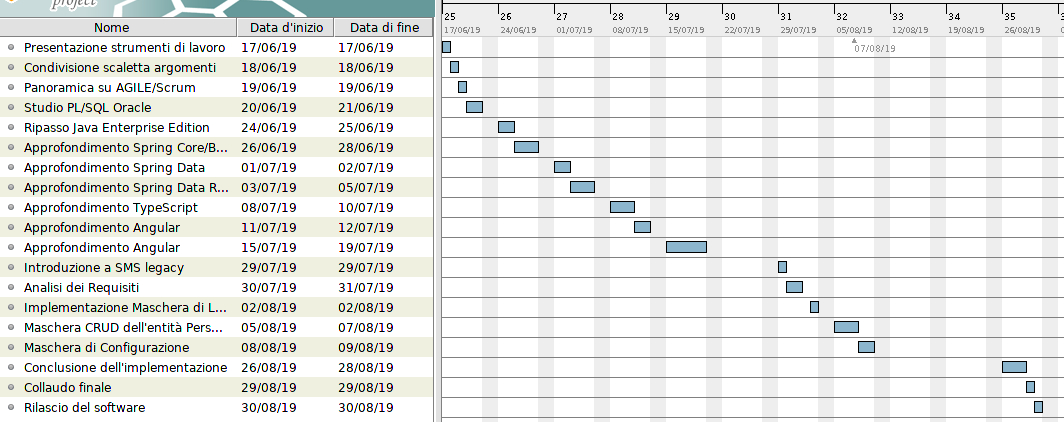
\includegraphics[width=1\columnwidth]{immagini/stage/gantt} 
	\caption{Diagramma di Gantt per la pianficazione dello stage}
	\label{figura:gantt-1}
\end{figure}

Sono presenti alcune settimane non aventi alcuna attività pianificata: ciò è dovuto a impegni pregressi pianificati dal sottoscritto e dalla chiusura dell'azienda per ferie.             % 
%% !TEX encoding = UTF-8
% !TEX TS-program = pdflatex
% !TEX root = ../tesi.tex

%**************************************************************
\chapter{Conclusioni}
\label{cap:conclusioni}
%**************************************************************

\section{COnsiderazioni generali}


\section{Obbiettivi raggiunti}

\section{Vantaggi riscontrati}

\section{Svantaggi riscontrati}

\section{Conoscenze acquisite}

\section{Sviluppi futuri}             %
%\appendix                               
%% !TEX encoding = UTF-8
% !TEX TS-program = pdflatex
% !TEX root = ../tesi.tex

%\epigraph{Citazione}{Autore della citazione}

%**************************************************************
\chapter{Altre tecnologie} \label{Appendice-1}
%**************************************************************

Lo scopo di questa sezione è fornire una panoramica delle tecnologie studiate durante il periodo di stage e previste nel piano di lavoro e che non hanno trovato un'applicazione concreta nel contesto del progetto SyncRec.\\
Tali tecnologie sono state incluse con il duplice scopo di ampliare il bagaglio di conoscenze del laureando e comprendere meglio l'architettura del progetto sul quale andavano fatti gli interventi concordati.

\section{Oracle PL/SQL} \label{plsql}
\textit{Oracle PL/SQL} è un linguaggio sviluppato da Oracle negli anni '80, si tratta di un linguaggio procedurale in grado di eseguire \textit{query SQL} insieme ad alcune strutture molto simili a quanto si può trovare in altri linguaggi procedurali (come \gls{Python} o \gls{ADA}).
PL/SQL fornisce le seguenti strutture:
\begin{itemize}
	\item Gestione degli errori;
	\item Tipizzazione dei dati;
	\item Le classiche strutture della programmazione (cicli, blocchi condizionali, funzioni etc.);
	\item Procedure;
	\item PSP (PL/SQL Server Pages);
	\item Piena integrazione con SQL(direttive DDL e DML sono disponibili in modo statico e dinamico)
\end{itemize}

\subsection{Struttura di uno script Oracle PL/SQL}
Uno \textit{script Oracle PL/SQL} è sempre suddiviso in al più tre parti:
\begin{itemize}
	\item \textbf{DECLARE:} si tratta di una sezione opzionale che contiene la dichiarazione di variabili, cursori e quant'altro;
	\item \textbf{BEGIN/END:} sezione obbligatoria che esegue le operazioni PL/SQL richieste;
	\item \textbf{EXCEPTION:} sezione facoltativa che si occupa della gestione degli errori all'interno dello \textit{script}.
\end{itemize}

All'interno del blocco \textit{DECLARE} è possibile definire inoltre due tipi di strutture: \textit{procedure} e \textit{funzioni}, dove l'unica differenza è che le seconde possono fornire valori in output tramite la keyword \textit{RETURN}.

Ogni script viene poi eseguito tramite la keyword \textit{Execute}.

\subsubsection{Cursori}
Per processare dichiarazioni SQL Oracle fornisce un area di memoria conosciuta come \textit{context area}, i \textit{cursori} costituiscono dei puntatori a tale area di memoria.\\
Il set di tuple risultanti da un'operazione SQL e puntato da un cursore è definito come l' \textit{Active Set}.\\
Per ogni operazione eseguita, Oracle instanzia un un cursore implicito, ed è inoltre possibile definire dei cursori \textit{custom} che processano le tuple una alla volta, applicando determinate trasformazioni definite dal programmatore.
I cursori vengono definiti nei blocchi PL/SQL e restringono la \textit{context area} tramite delle classiche \textit{SELECT} in SQL.\\
I cursori, in ultima analisi, sono uno strumento molto potente per manipolare i risultati delle operazioni SQL, tuttavia oggi risultano piuttosto datati se si considerano le potenzialità dei moderni \gls{framework} e la loro capacità di processare i dati contenuti nei database.

\section{Archittetture a microservizi}\label{micro}
Un’architettura basata su microservizi viene aplicata nella realizzazione di un’applicazione, essa è costituita da componenti indipendenti che eseguono ciascun processo applicativo come un \textbf{servizio}.\\
Tali servizi comunicano attraverso un’interfaccia ben definita che utilizza API leggere. Ciò risulta vantaggioso poiché ciascun componente viene eseguito in modo indipendente, e ciascun servizio può essere aggiornato, distribuito e ridimensionato per rispondere alla richiesta di funzioni specifiche di un’applicazione.\\
Ciascun servizio è progettato per una serie di capacità e si concentra sulla risoluzione di un problema specifico. Se, nel tempo, gli sviluppatori aggiungono del codice aggiuntivo a un servizio rendendolo più complesso, il servizio può essere scomposto in servizi più piccoli.

Tra le principali qualità di un'architettura a microservizi troviamo:

\begin{itemize}
	\item \textbf{Agilità:}I microservizi promuovono le organizzazioni di team indipendenti di dimensioni ridotte che diventano proprietari del servizio che gestiscono. Ciò comporta tempi di sviluppo minori in contesti ridotti e ben delineati.
	\item \textbf{Scalabilità e flessibilità}I microservizi consentono di scalare ciascun servizio in modo indipendente per rispondere alla richiesta delle funzionalità che l'applicazione supporta. Ciò permette ai team di adattare in modo corretto l’infrastruttura rispetto alle necessità, con la possibilità di monitorare accuratamente i servizi nel caso in cui essi rilevino un aumento del flusso di transazioni.
	\item \textbf{Semplicità di distribuzione}I microservizi supportano l’integrazione continua e la distribuzione continua; l'apporto di modifiche errate non inficia sul corretto funzionamento generale dell'applicazione e gli errori influiscono di meno sul costo delle operazioni. 
	\item \textbf{Libertà tecnologica} L'utilizzo di un'architettura a microservizi non è legata a un particolare \textit{stack} tecnologico: i team di sviluppo hanno piena libertà nella scelta e adozione delle tecnologie da utilizzare nel corso dello sviluppo di un progetto.
	\item \textbf{Codice riutilizzabile} La suddivisione in moduli ben delineati ha il grande vantaggio di rendere il codice riutilizzabile; è possibile quindi utilizzare moduli e servizi pienamente funzionanti per lo sviluppo di componenti aggiuntivi.
	\item \textbf{Resilienza} A differenza di quanto accade in un'architettura monolitica, un errore non è in grado in alcun modo di pregiudicare il corretto funzionamento di un'applicazione; ciò è dovuto alla natura indipendente dei servizi per come sono concepitis.
	
\end{itemize}             % Appendice A

%**************************************************************
% Materiale finale
%**************************************************************
\backmatter
\printglossaries
%% !TEX encoding = UTF-8
% !TEX TS-program = pdflatex
% !TEX root = ../tesi.tex

%**************************************************************
% Bibliografia
%**************************************************************
\cleardoublepage
\begin{thebibliography}{99}
	\bibitem{site:sqlserverpricing}
	\textit{Prezzi di SQL Server - consultato 13/09/2018}\\
	\url{https://bit.ly/2rECrAS}
	
	\bibitem{site:sqlcomparison}
	\textit{Studio comparativo sulle performance di SQL Server PostgreSQL Oracle XE e MySQL - consultato 13/09/2018}\\
	\url{https://bit.ly/2MtTE8e}
		
	\bibitem{site:svnvsgit}
	\textit{Differences Between Git and SVN  - consultato 13/09/2018}\\
	\url{https://bit.ly/2p4NzWI}

	\bibitem{site:crociereregalo}
	\textit{URL del sito CrociereRegalo (parte OTA)}\\
	\url{https://www.crociereregalo.it}
		
	\bibitem{site:dataexchange}
	\textit{URL del sito CrociereRegalo (parte DataExchange)}\\
	\url{https://data.crociereregalo.it}
	
	\bibitem{site:sviluppo-crociereregalo}
	\textit{URL del sito di sviluppo CrociereRegalo (parte OTA)}\\
	\url{http://primaretetest.webpd.it/crociereregalo}
	
	\bibitem{site:sviluppo-dataexchange}
	\textit{URL del sito di sviluppo CrociereRegalo (parte DataExchange)}\\
	\url{http://primaretetest.webpd.it/dataExchange}
	
	% Citazioni da glossario
	\bibitem{site:wikipediaIDE}
	\textit{Integrated development environment - consultato 18/09/2018}\\
	\url{https://bit.ly/2p4NzWI}

	\bibitem{site:api}
	\textit{Cosa sono le API e a cosa servono - consultato 18/09/2018}\\
	\url{https://bit.ly/2xm5qgq}

	\bibitem{site:webservice}
	\textit{Web Services Architecture - consultato 18/09/2018}\\
	\url{https://www.w3.org/TR/ws-arch/\#introduction}

	\bibitem{site:seo}
	\textit{Guida SEO all’Ottimizzazione per Motori di Ricerca - consultato 18/09/2018}\\
	\url{https://bit.ly/2QGWt9x}
	
	% Citazioni da glossario
	\bibitem{book:mvc}
	\textit{Advanced ActionScript 3 with Design Patterns}\\
	Joe Lott, Danny Patterson\\
	\textit{Pagina 46}

	\bibitem{site:rpc}
	\textit{Remote Procedure Call - consultato 18/09/2018}\\
	\url{https://bit.ly/2rjaUVo}

	\bibitem{site:soap}
	\textit{Remote Procedure Call - consultato 18/09/2018}\\
	\url{https://www.w3schools.com/xml/xml_soap.asp}	

	\bibitem{site:dbms}
	\textit{Data Base Management System - consultato 18/09/2018}\\
	\url{https://bit.ly/2HECZMV}

	\bibitem{site:rdbms}
	\textit{RDBMS - consultato 18/09/2018}\\
	\url{https://bit.ly/1MLo1Q4}
	
	\bibitem{site:framework}
	\textit{Framework - consultato 18/09/2018}\\
	\url{https://bit.ly/2QGe2Gr}
	

	\bibitem{site:dom}
	\textit{JavaScript HTML DOM - consultato 18/09/2018}\\
	\url{https://www.w3schools.com/js/js_htmldom.asp}	
	

	\bibitem{site:json}
	\textit{Introducing JSON - consultato 18/09/2018}\\
	\url{https://www.json.org/}


	\bibitem{site:ajax}
	\textit{AJAX Introduction - consultato 18/09/2018}\\
	\url{https://www.w3schools.com/xml/ajax_intro.asp}
	
	% Fine citazioni da glossario
\end{thebibliography}




\end{document}
